\documentclass[aspectratio=169]{beamer}
\usepackage{xcolor}
%\documentclass[handout]{beamer} % turns on handout mode to surpress the \pause
\usetheme[progressbar=frametitle]{metropolis}
\usepackage{appendixnumberbeamer}
\usepackage{changepage}
\usepackage{pgfpages}
\usecolortheme{beaver}
\setbeamertemplate{footline}[frame number]
\setbeamerfont{footnote}{size=\tiny}

% turn off/on showing notes in the presentation
\setbeameroption{show notes on second screen}
%\setbeameroption{hide notes}
\setbeamertemplate{note page}[plain]

\definecolor{BlueGreen}{cmyk}{0.85,0,0.33,0}
\definecolor{RawSienna}{cmyk}{0,0.72,1,0.45}

\title{Ryan and Sudarshan 2020 - Rationing the Commons}
\author{Yixin Sun}
\institute{\emph{EEE Presentation}}
\date{\today}

\begin{document}
\begin{frame}
\titlepage
\end{frame}


\section{Introduction}
\begin{frame}
    \frametitle{Motivation}
    \begin{itemize}
        \item Economic development often has led to the mass depletion of natural resources (fisheries, hunting, forests, and of course water) \pause 
        \item India is now the largest user of groundwater in the world, extracting more in a year than in the US and China combined \pause 
        \item Economists have tools (pricing, property rights) that should lead to efficient outcomes \pause
        \item But do we balance equity and efficiency? \pause 
    \end{itemize}

    Research question: how does the current groundwater rationing system in India balance the trade-off between efficiency and equity?
\end{frame}

\begin{frame}
\frametitle{Context: Common Pool Problem in Indian Groundwater}
\begin{figure}[H]
    \centering
    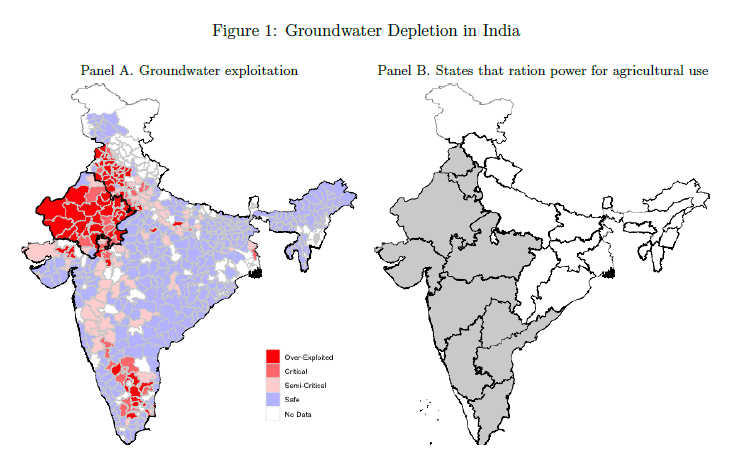
\includegraphics[height = 2.7in]{fig1.png}
\end{figure}

\note{
{\footnotesize
\begin{itemize}
    \item The spread of groundwater irrigation was instrumental in ushering in the Green Revolution of the 1960s and 1970s. This led to huge productivity growth in India, but also huge depletions of groundwater
    \item Rajasthan, the area of study in this paper, has an extraordinary concentration of districts withover-exploited groundwater and as a state is extracting groundwater at 137\% of the rate that can naturally be recharged. (Point to Rajasthan, which is the area outlined in black on the left hand side)
    \item Primary method government oversight is Use rationing of electricity to limit how much water farmers can extract. We can see this on the left hand panel, which shades the states in India that use a rationing regime in supplying power for farmers
\end{itemize}
}}
\end{frame}



\begin{frame}
\frametitle{Weitzman Detour}
Weitzman (1977): Is the Price System or Rationing More Effective in Getting a Commodity to Those Who Need It Most? 

\small
\textit{"There is a class of commodities whose just distribution is sometimes viewed as a desirable end in itself, independent of how society may be allocating its other resources. While it is always somewhat arbitrary where the line should be drawn, such "natural right goods" as basic food and shelter, security, legal aid, military service, medical assistance, education, justice, or even many others are frequently deemed to be sufficiently vital in some sense to give them a special status. The principal of limited dimensional equity in the distribution of a commodity is an open violation of consumer sovereignty."}


\note{
{\footnotesize
\begin{itemize}
    \item We've seen Weitzman's famous Prices vs. Quantities paper in class, but Weitzman actually also has a paper called "Is the Price System or Rationing More Effective in Getting a Commodity to Those Who Need It Most". And I'll just share with you the quote from the paper that outlines why he sets up this other framework to think about "natural right goods" 
\end{itemize}
}}
\end{frame}

\begin{frame}
    \frametitle{Weitzman Detour: Model}
    \begin{enumerate}
        \item Measures each consumer's relative need vs. ideal allocation based on that need. \pause
        \item Social objective function: quadratic loss between ideal and actual allocations \pause
        \item Limited-information assumption: government needs to choose an allocation system without perfect information on where individuals lie on a distribution
    \end{enumerate}
    
    
    \note{
    {\footnotesize
    \begin{itemize}
        \item Measures each consumer's relative need vs. ideal allocation based on that need. Note he uses "need" rather than "preference" because he is specifically thinking about goods such as water rather than widgets, because these are goods where distributional issues are important 
        \item The second is the social objective function, which is the quadratic loss between ideal and actual allocations
        \item  Limited-information assumption: government needs to choose an allocation system without perfect information on where individuals lie on a distribution. Since everyone has read the paper, this definitely sounds like the setting that Ryan and Sudarshan are studying. 
    \end{itemize}
    }}
\end{frame}

\begin{frame}
    \frametitle{Weitzman Detour: Results}
   
    If people's needs are more widely dispersed or if the society is relatively egalitarian $\rightarrow$ price mechanism \pause

    \vspace{1.3cm}

    If people's needs are quite uniform or there is great income inequality $\rightarrow$ rationing mechanism
    
    
    \note{
    {\footnotesize
    \begin{itemize}
        \item If people's needs are more widely dispersed or if the society is relatively egalitarian, then a pricing mechanism works better
        \item If people's needs are quite uniform or there is great income inequality, then a rationing mechanism is better. 
        \item I think it's important to think about how this differs from a direct applicaiton of Prices vs. Quantities framework. If I were to think about this problem after I watched Ryan's lectures but before I read the rationing the commons paper, I think my train of thought would've been, "demand elasticity of water tends to be pretty big in the literature, so the marginal benefits curve is pretty flat, so if I apply Weitzman 1974, then we should use a pricing mechanism to solve the common resource problem in India". 
        \item But that's not the conclusion you'd probably reach using Weitzman 1977 (don't ask me about the math though). I think the intuition here is that Weitzman's notion of need is affected by income and your own idiosyncratic need for a good. So when there is no income inequality, prices are effective at allocating the good because willingness to pay is an efficient measurement of the need of an individual. However, when there is huge income inequality, a rationing scheme essentially prevents those with larger incomes from monopolizing consumption of the commodity in question
    \end{itemize}
    }}
\end{frame}

%%%%%%%%%%%%%%%%%%%%%%%%%%%%%%%%%%%%%%%%%%%%%%%%%%%%%%%%%%%%%%%%%%%%%%%%%%%%%%%%
\section{Model of agricultural production under rationing}
%%%%%%%%%%%%%%%%%%%%%%%%%%%%%%%%%%%%%%%%%%%%%%%%%%%%%%%%%%%%%%%%%%%%%%%%%%%%%%%%
\begin{frame}
    \frametitle{Modelling the Optimal Ration} 
    \begin{gather*}
        \underbrace{\sum_{i} \frac{d \widetilde{\Pi}_{i}\left(W_{i}\left(\bar{H}^{*}, D_{i}\right)\right)}{d \bar{H}^{*}}}_{\text {Marginal benefit }}=\underbrace{\sum_{i} c_{E} P_{i}+\rho \frac{P_{i}}{D_{i}} \lambda_{W}}_{\text {Marginal social cost }}
    \end{gather*} 

    \begin{center}
        Farmer profits = Direct cost of elec. + Opportunity cost    
    \end{center}

\note{
    {\footnotesize
    \begin{itemize}
        \item Paper begins by modelling agricultural production with groundwater. 
        \item Farmers are heterogeneous in productivity and in factor endowments. 
        \item Under rationing, markets clear on quantity
        \item Here we are considering the state's problem: they are maximizing total surplus, taking as given the price of electricity, and they have to choose a ration, $\bar{H}$. So we get the familiar FOC for the optimal ration in the slide
        \item Efficient ration balances the marginal social benefit of increasing the ration against the marginal social cost 
        \item The benefits are the additional profits farmers earn when the state increases the ratio, which allows farmers to extract more water 
        \item The marginal cost has two parts. The first is the cost of generating and distributing the additional electricity that farmers use when the state increases the ration. The second is the opportunity cost of water extraction due to the externality: if a farmer uses water today, the water level will fall, and the cost of water extraction tomorrow will rise. 
        \item An important result here is that even an optimal ration distorts allocation of water and lowers surplus because it is forcing heterogeneous farmers to  have the same level of power use. 
    \end{itemize}
    }}
\end{frame}

\begin{frame}
    \frametitle{Sufficient Statistic for Electricity Ration} 
    \begin{gather*}
        W_{i}\left(H_{i}, D_{i}\right)=\rho \frac{P_{i} H_{i}}{D_{i}} 
    \end{gather*} \
    \begin{gather*}
        \sum_{i} \frac{d \widetilde{\Pi}_{i}\left(W_{i}\left(\bar{H}, D_{i}\right)\right)}{d \bar{H}} = \sum_{i}-\frac{d \widetilde{\Pi}_{i}}{d D_{i}} \frac{D_{i}}{H_{i}}
    \end{gather*}
\note{
    {\footnotesize
    \begin{itemize}
        \item The above equation is intuitive - we want to balance marginal benefits and marginal cost
        \item But we can't measure marginal benefit directly because the ration does not vary. Also, as shown by their agricultural survey, the ration binds for almost all farmers, so we can't see marginal willingness-to-pay 
        \item But they know that water extraction is dictated by this water extraction function. So they can replace the increase in water due to a change in the ration with the increase in water due to a change in depth. So the marginal return to depth is a sufficient statistic for the benefit of an increased electricity ration. They use plausibly exogenous variation in groundwater conditions, based on the geology of aquifers, to estimate farmer's return to water. 
    \end{itemize}
}}

\end{frame}

%%%%%%%%%%%%%%%%%%%%%%%%%%%%%%%%%%%%%%%%%%%%%%%%%%%%%%%%%%%%%%%%%%%%%%%%%%%%%%%%
\section{Calculating Marginal Benefits v Costs}
%%%%%%%%%%%%%%%%%%%%%%%%%%%%%%%%%%%%%%%%%%%%%%%%%%%%%%%%%%%%%%%%%%%%%%%%%%%%%%%%
\begin{frame}
    \frametitle{Hedonic IV Regression to Estimate Marginal Benefits}
    \label{hedonic}
    \begin{align*}
        \Pi_{i c} &=\beta_{o}+D_{i} \beta_{1}+X_{i c}^{\prime} \beta_{2}+\alpha_{s}+\alpha_{p}+\epsilon_{i c} \\
        D_{i} &=\delta_{0}+Z_{i}^{\prime} \delta_{1}+\eta_{i c}
    \end{align*}

    \begin{center}
        \textcolor{RawSienna}{Coefficient of interest: $\beta_1 = \frac{d\Pi}{dD}$}
    \end{center}

    \vfill
    \rightline{\hyperlink{endogeneity}{\beamerbutton{Discussion}}}

    \note{
    {\footnotesize
    \begin{itemize}
        \item To estimate the marginal benefit of more water, the authors regress profits on well depth, along with controls for farmer and crop characteristics, and fixed effects. 
        \item However, OLS could suffer from endogeneity or omitted variable bias, say if more profitable farmers are able to get land with less water depth. 
        \item Solution: use geological characteristics as an instrument for well depth
    \end{itemize}
    }}
\end{frame}

\begin{frame}
    \frametitle{Results of Hedonic Regressions}
    \begin{figure}[H]
        \centering
        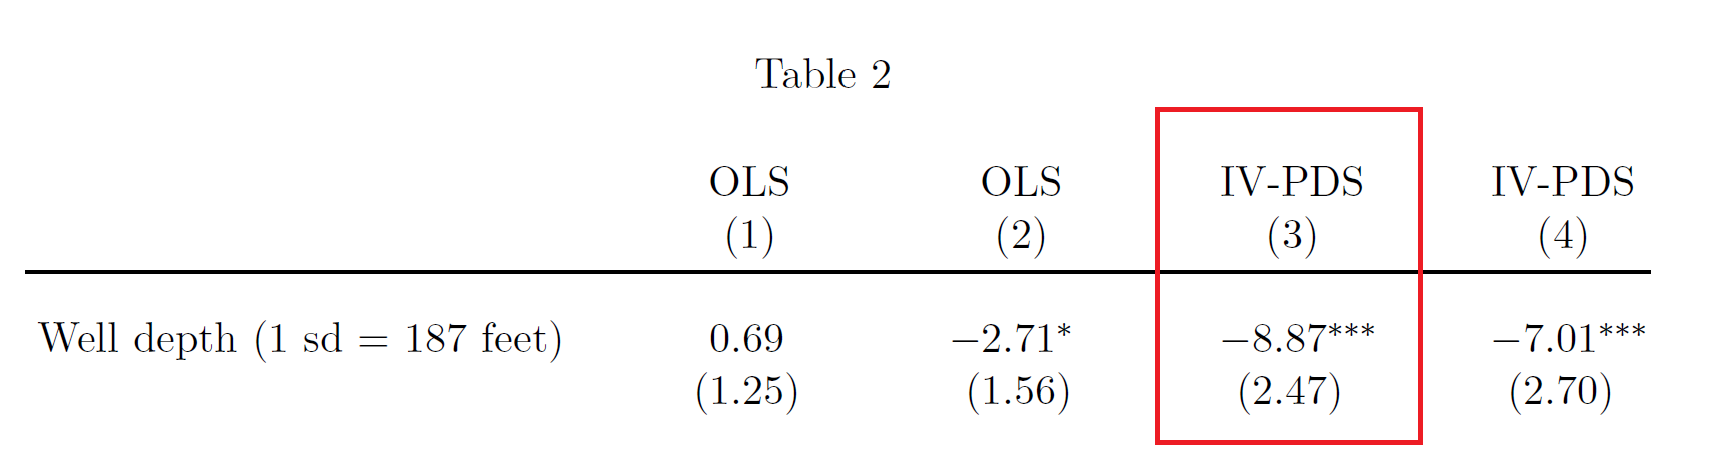
\includegraphics[height = 1.3in]{table2.png}
    \end{figure}
    \note{
        {\footnotesize
        \begin{itemize}
            \item In their preferred specification, they find that a one standard deviation increase in depth decreases profit by 8,900 rupees per hectare in the dry season
            \item This reduction is about 14\% of output per hectare, or 15\% of household income for the average farmer
            \item So by these estimates, the amount of water is incredibly valuable for farmers
        \end{itemize}
        }}
\end{frame}

\begin{frame}
    \label{fig4}
    \frametitle{Comparing Marginal Benefits and Costs of Ration}
    \begin{figure}[H]
        \centering
        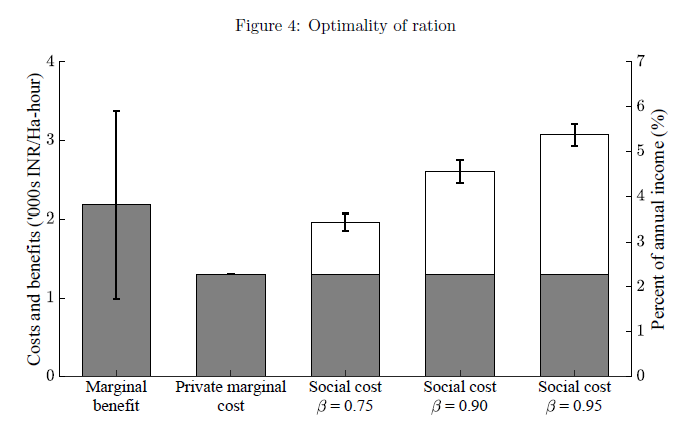
\includegraphics[height = 2.5in]{fig4.png}
    \end{figure}
    \rightline{\hyperlink{future}{\beamerbutton{Discussion}}}
    \note{
        {\footnotesize
        \begin{itemize}
            \item The next step is to estimate the opportunity cost. This was the $\lambda_w$ that we saw from before, which depends on how water extraction today affects groundwater levels tomorrow as well as on the returns to water in agriculture and the discount rate. 
            \item They use a simplified dynamic version of their production model to estimate this
            \item Figure 4 translates these comparisons into comparisons of marginal benefits nad marginal costs. 
            \item The first bar translates the results from the regression, the $\beta_1$ they found, and finds that a one-hour increase in power supply increases farmer profits by 2,200 rupees per hactare. The remaining bars show the costs, where the gray region is the direct cost of power, and the top white bar is the cost of water for three different discount factors
            \item This figure implies that on average, farmers are not using too much water, and that the ration is roughly efficient 
        \end{itemize}
        }}
\end{frame}


%%%%%%%%%%%%%%%%%%%%%%%%%%%%%%%%%%%%%%%%%%%%%%%%%%%%%%%%%%%%%%%%%%%%%%%%%%%%%%%%
\section{Structural Estimation and Counterfactuals}
%%%%%%%%%%%%%%%%%%%%%%%%%%%%%%%%%%%%%%%%%%%%%%%%%%%%%%%%%%%%%%%%%%%%%%%%%%%%%%%%
\begin{frame}
    \frametitle{Structural Model of Agricultural Production}
    \begin{gather*}
        y_{i c}=\alpha_{L} l_{i c}+\alpha_{X} x_{i c}+\alpha_{K} k_{i c}+\alpha_{W} w_{i c}+\omega_{Y i c} \\
        \text{farmer $i$ planting crop $c$}
    \end{gather*}

    \begin{align*}
        \omega_{Y i c}=\underbrace{\overbrace{W_{E i c} \beta_{E}}^{\text{known output shifters}}+\overbrace{\omega_{i c}}^{\text{farmer-specific shock}}}_{\text{obs. by farmer}}+\underbrace{\epsilon_{Y i c}}_{\text{unobs. shock at harvest}}
    \end{align*}
    \note{
        {\footnotesize
        \begin{itemize}
            \item Even though the rationing may be about right, we discussed on a previous slide that even a perfectly set ration imposes allocative inefficiencies, because everyone has the same ration, regardless of productivity. 
            \item To compare rationing to Pigouvian pricing, they estimate a structural model of agricultural production
            \item Assume a Cobb-Douglas function shown here, with yields a residual that has several components. The first term consists of known output shifters. The second is a farmer-specific shock. Both these are observed by the farmer early in the season and hence input choies are endogenous to these terms. The third is an unobservable shock at harvest. The econometrician only observes $W_{Eic}$. 
            \item They run this production function as a regression, again using an instrumental variable approach to account for endogeneity of input choices to productivity. 
            \item From the residuals of their regression, the authors can calculate the implied TFP for farmers. 
        \end{itemize}
        }}
\end{frame}

\begin{frame}
    \frametitle{Model Estimates and Dispersion of Shadow Costs}
    \begin{figure}[H]
        \centering
        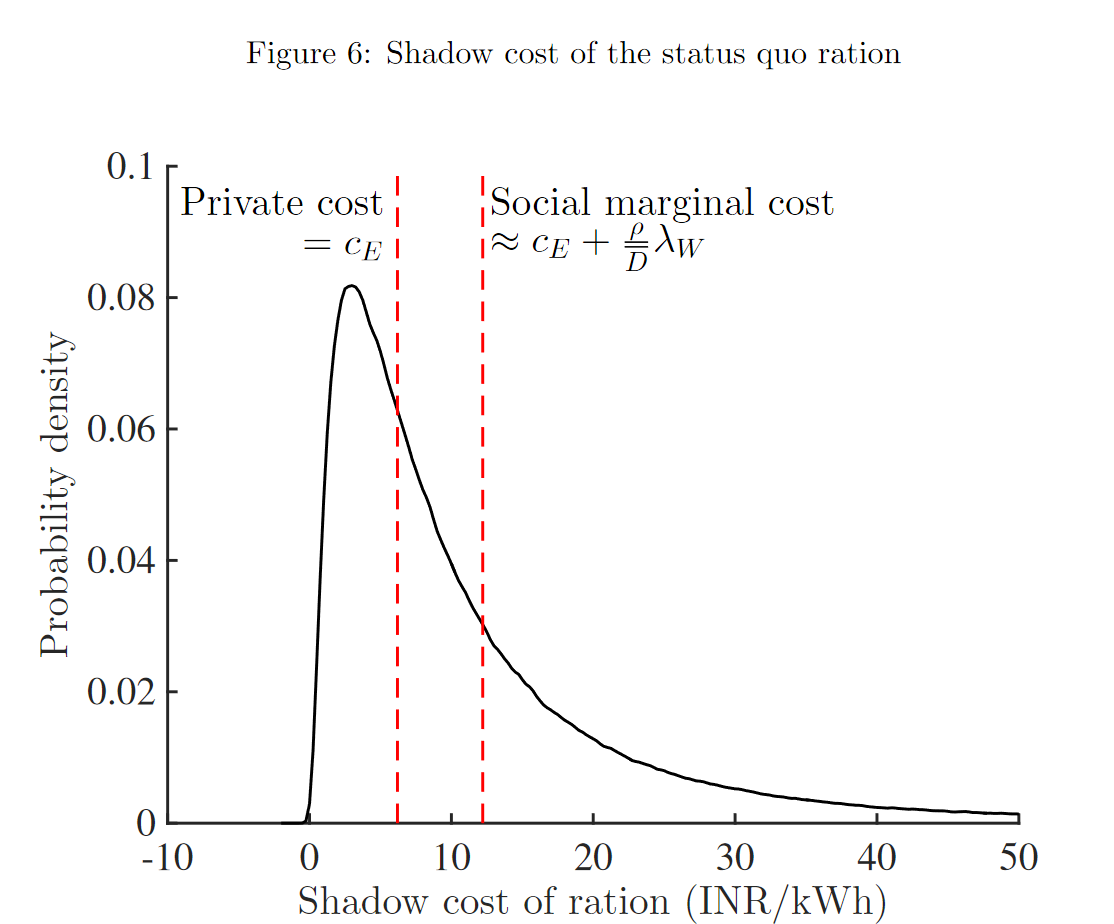
\includegraphics[height = 2.7in]{fig6.png}
    \end{figure}
    \note{
        {\footnotesize
        \begin{itemize}
            \item The model estimates then allow the authors to calculate the shadow cost of ration for each farmer 
            \item This shadow cost is the price of electricity such that each farmer, if unconstrained, would optimally choose to use the rationed amount of water. 
            \item They graph these shadow costs in figure 6. We see that about 2/3 of the farmers have a shadow cost less than social marginal cost. But we have this long right tail of farmers with extremely high shadow costs. 
            \item This high dispersion gives us an illustration of there being a high degree of misallocation of water across farmers
        \end{itemize}
    }}
\end{frame}

\begin{frame}
    \frametitle{Running Counterfactual Regimes and Transfers}
    \label{counterfactuals}
    \begin{columns}[t]

        \begin{column}{0.48\textwidth}
        \color{BlueGreen}\rule{\linewidth}{4pt}
        Counterfactual Regimes
        \begin{enumerate}
            \item Ration set at optimal, rather than 6 hours
            \item Pricing regimes instead of ration, sets price of electricity at private marginal cost
            \item Pigouvian regime $\rightarrow$ sets price of electricity at social marginal cost
        \end{enumerate}
        \end{column}
        
        \begin{column}{0.48\textwidth}
        \color{RawSienna}\rule{\linewidth}{4pt}
        Transfer Methods
        \begin{enumerate}
            \item Flat (uniform) transfers across farmers
            \item Transfers on basis of land size
            \item Transfers on basis of pump capacity
        \end{enumerate}
        \end{column}
        
    \end{columns}

    \vfill
    \rightline{\hyperlink{pigouvian}{\beamerbutton{Equations}}}
\end{frame}

\begin{frame}
    \frametitle{Counterfactual Regimes Results}
    \begin{figure}[H]
        \centering
        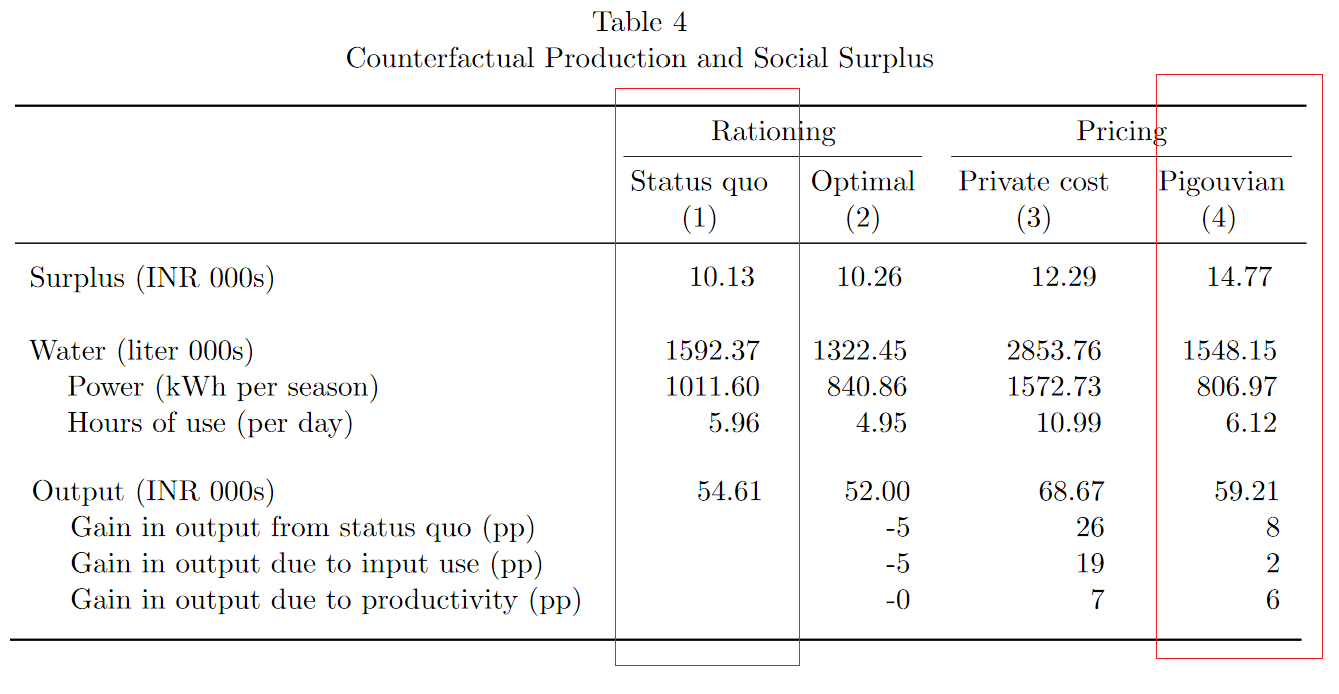
\includegraphics[height = 2.7in]{table4.png}
    \end{figure}
    \note{
        {\footnotesize
        \begin{itemize}
            \item Column 1 is status quo 6 hour ration Column 2 is the optimal ration. Column 3 is pricing at private costs, and column 4 is Pigouvian pricing.
            \item We see that the ration is at roughly the efficient level - column two here sets the optimal ration at 5 hours 
            \item We see large efficiency costs with rations. If you look at the mean surplus in column 1, we can get a 50\% increase under Pigouvian pricing. The authors calculate that this gain in surplus would equal 12\% of the annual household income, so these potential gains are huge!
            \item The other thing to note here is that the surplus gains under Pigou are because of increases in productivity rather than water conservation. We see that average water extraction is nearly the same under Pigou. But if we look at gains in output in the last section of rows, 6 of the 8 percentage point increases in output are due to higher productivity rather than input use 
            \item 
        \end{itemize}
    }}
\end{frame}


\begin{frame}
    \frametitle{Distributional Impacts of Pigouvian Reform}
    \begin{figure}[H]
        \centering
        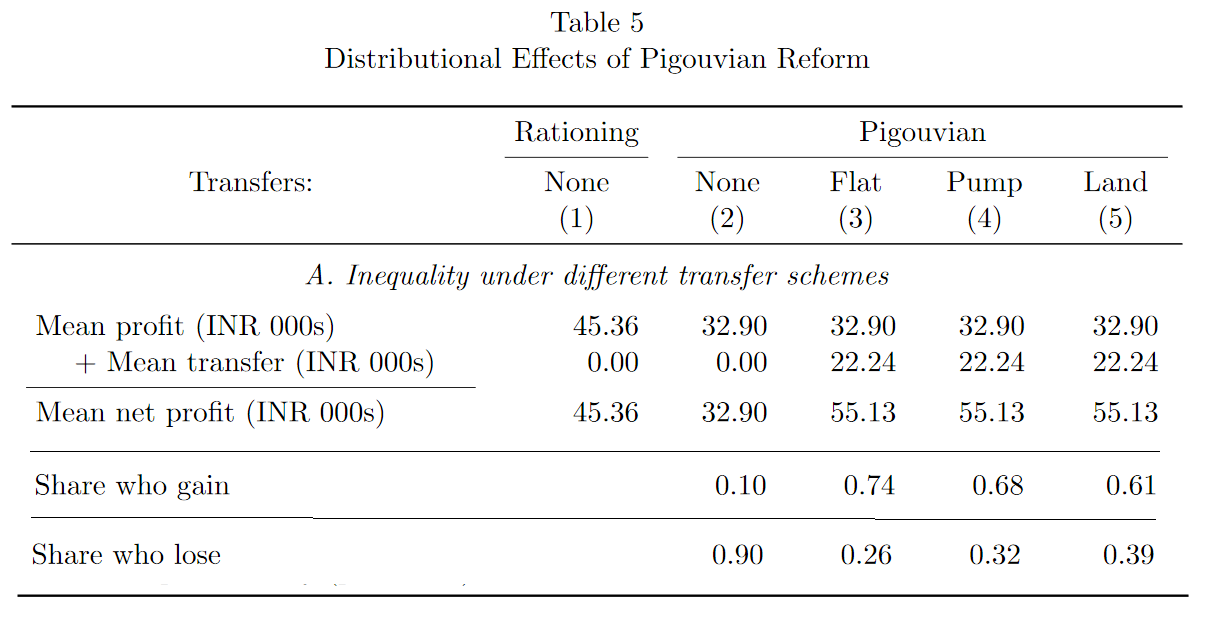
\includegraphics[height = 2.7in]{table5.png}
    \end{figure}
    \note{
        {\footnotesize
        \begin{itemize}
            \item But this is potential surplus gain is not the end of the story. The author ends this paper by studying the distributional impacts of Pigouvian reform. 
            \item Column 1 here gives status quo results, and the next four compares the status quo to the Pigouvian regime under the different transfer mechanisms we discussed in the previous slide. 
            \item We see that without transfers, most farmers lose out under Pigouvian pricing 
            \item With flat transfers, 74\% of farmers gain, which is substantial but not a Pareto improvement. And what's important to note is that those who lose tend to be farmers with high ex ante profits, land, and productivity, and deeper wells. So this scheme actually mostly harms productive, moderate landholders in areas with severe groundwater depletion.
            \item And in the last two columns, we see that targetting transfers based on pump capacity or land size actually hurts more farmers than the flat fee transfer scheme. The intuition here is that targeting mainly shifts the burden of losses, because they end up spending a large part of the budget on large farmers who would've been profitable even without transfers. 
            \item This highlights one of the paper's key points: productivity is the key determinant of gains from reform, but the state cannot target transfers on productivity, which means Pigouvian regimes still leave a large number of farmers worse off. 
        \end{itemize}
    }}
\end{frame}


\begin{frame}
    \frametitle{Summary}
    \begin{itemize}
        \item On average, the current 6-hour ration is set at the roughly efficient level
        \item With farmer heterogeneity, even the optimal ration produces allocative inefficiency
        \item Pigouvian pricing would lead to large increases in social surpluses, but about 90\% of farmers would lose out if no transfers are given 
        \item Even with transfers, significant portions of farmers would still be worse off 
    \end{itemize}
\end{frame}

%%%%%%%%%%%%%%%%%%%%%%%%%%%%%%%%%%%%%%%%%%%%%%%%%%%%%%%%%%%%%%%%%%%%%%%%%%%%%%%%
\section{Discussion} 
%%%%%%%%%%%%%%%%%%%%%%%%%%%%%%%%%%%%%%%%%%%%%%%%%%%%%%%%%%%%%%%%%%%%%%%%%%%%%%%%
\begin{frame}
    \frametitle{Musings}
    \begin{itemize}
        \item Appreciate a comparison between efficiency and distribution
        \item Comparing current policy to realistic policies that government could take $\rightarrow$ Coase would be proud!
        \item Extremely well written and easy to understand, even with all the moving parts 
    \end{itemize}
\end{frame}

\begin{frame}
    \frametitle{Importance of This Paper}
    \begin{itemize}
        \item Agriculture is about 16\% of India's GDP, but it's a huge portion of consumer surplus
        \item About 60\% of Indian population works in the agriculture sector
        \item India's agricultural output accounts for about 7\% of world agricultural output
        \item How we use water today has many feedback components that are made worse with climate change
        \item Direct Benefit Transfers (DBT) of Electricity subsidies 
    \end{itemize}
    \note{
        {\footnotesize
        Then climate change is bringing in a new slew of issues surrounding water and agriculture. 
        \begin{itemize}
            \item earlier spring melt - lost storage from snow pack
            \item More variable precipitation; makes existing storage of water less usable, and more frequent and severe drought
            \item These issues lead to groundwater depletion and less groundwater recharge
            \item implication is that irrigation and technology improvements are very unlikely to be the adaptation strategy for climate change $rightarrow$ we need to think about what government intervention looks like
        \end{itemize}
        Indian government proposed a Direct Benefit Transfers of Electricity plan, where farmers would pay the bill for the power consumed for farming. After that, they get the subsidy in their bank accounts for the hours they do not use electricity. So farmers can select into using all of their electricity ration, or cut back and receive a cash transfer, thereby implicitly selecting on productivity. 
    }}
\end{frame}

\begin{frame}
    \frametitle{How Should We Think About the Future?}
    \label{future}
    \begin{itemize}
        \item Paper found that the rationing status quo seems close to being efficient, but hard to reconcile this with the fact that "Rajasthan as a state is extracting groundwater at 137\% of the rate that can naturally be recharged." \pause 
        \item Are they picking the right discount rate? \hyperlink{fig4}{\beamerbutton{Fig. 4}} \pause
        \item Method of estimating costs does not incorporate the feedback components discussed
    \end{itemize}
\end{frame}

\begin{frame}
    \frametitle{Instrument Variable Exclusion Restriction}
    \label{endogeneity}
    \begin{itemize}
        \item To estimate marginal benefits from more water, authors use geological features as an instrument for water depth. \hyperlink{hedonic}{\beamerbutton{IV}}
        \item How does this get rid of the endogeneity concern?
    \end{itemize}
    \note{
    {\footnotesize
    \begin{itemize}
        \item 
    \end{itemize}
    }}
\end{frame}

\begin{frame}
    \frametitle{Possible Extension: Marginal Benefits in Panel Data}
    This paper estimated marginal benefits using cross-sectional data because "it can recover long-run elasticities of profit with respect to water, net of farmer adaptation"

    What are the implications if we take into account that farmers can adapt or switch crops when the government sets a high enough ration?
\end{frame}

\begin{frame}
    \frametitle{Smaller Questions:}
    \begin{itemize}
        \item Do farmers usually pay their electricity bills? Perhaps pricing isn't feasible also because no one actually pays for electricity
        \item Does quality of electricity matter here/is it lumped in with productivity?
        \item Are microgrids or alternative energy sources used to get around the ration?
        \item In equation (9), why is it important to include $W_{Eic}$ in the residual if those are observable?
    \end{itemize}
\end{frame}

\begin{frame}
    \frametitle{Extra Slide: Pigouvian vs Rationing}
    \label{pigouvian}
    Pigouvian Regime: $p_{E}^{*}=\underset{p_{E}}{\arg \max } \sum_{i} \mathbb{E}\left[\widetilde{\Pi}_{i}\left(p_{E}\right)-c_{E} P_{i} H_{i}\left(p_{E}\right)-\rho_{i} \frac{H_{i}\left(p_{E}\right)}{D_{i}} \lambda_{W}\right]$

    Rationing Regime: $\bar{H}^* = \underset{\bar{H}}{\arg \max}\sum_{i}\left[\widetilde{\Pi}_{i}\left(W_{i}\left(\bar{H}, D_{i}\right)\right)-c_{E} P_{i} \bar{H}-\rho \frac{P_{i}}{D_{i}} \bar{H} \lambda_{W}\right]$
    \vfill
    \rightline{\hyperlink{counterfactuals}{\beamerbutton{Counterfactuals}}}
\end{frame}
\end{document}

%Other template that's nice https://www.overleaf.com/project/5e78d1da3875680001cc8c73























